% @Author: Ram Krishna Sharma
% @Date:   2021-05-18
% @Last Modified by:   Ram Krishna Sharma
% @Last Modified time: 2021-05-27
\subsubsection{Categorization}
\label{subsubsec:Categorization}

Events falling into the Fully-hadronic category are categorized in a similar fasion as described in Section \ref{subsubsec:SLCategorization} for the Semi-leptonic channel, but with the addition of a selection on the bb$\gamma\gamma$ killer score. 

% The categorization is performed in a similar way as described in sec.~\ref{subsubsec:SLCategorization}, for Semi-Leptonic channel.

The expected signal region yields background processes, simulated with MC, and HH signal, both scaled to the Run 2 luminosity of 137 $fb^{-1}$ (the estimated luminosity value at the time of training), are shown in Figure \ref{fig:FH_DnnScore}
for the WW$\gamma\gamma$ identifier score.

\begin{figure}[!htbp]
  \centering
  % 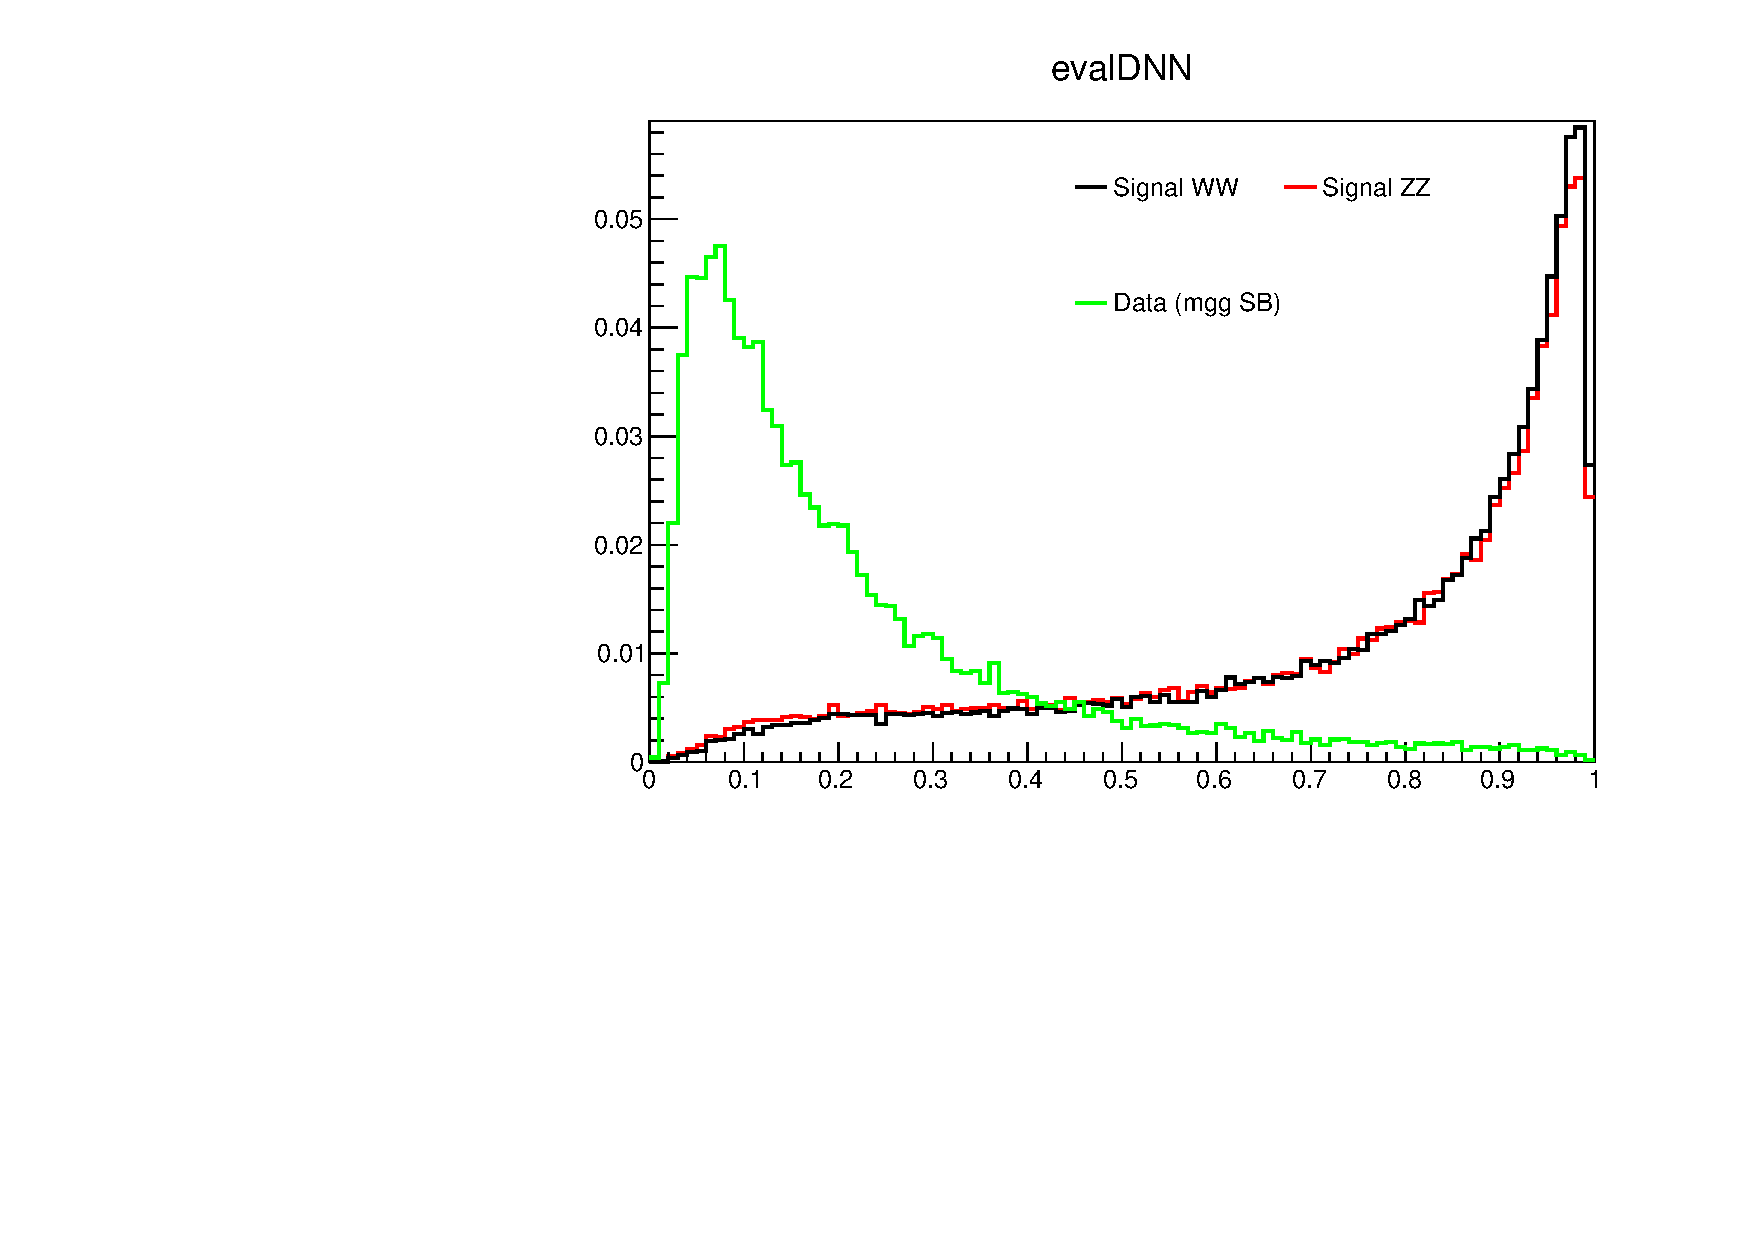
\includegraphics[scale=0.6]{Sections/HHWWgg/images/FH_DNN/evalDNN.pdf}
  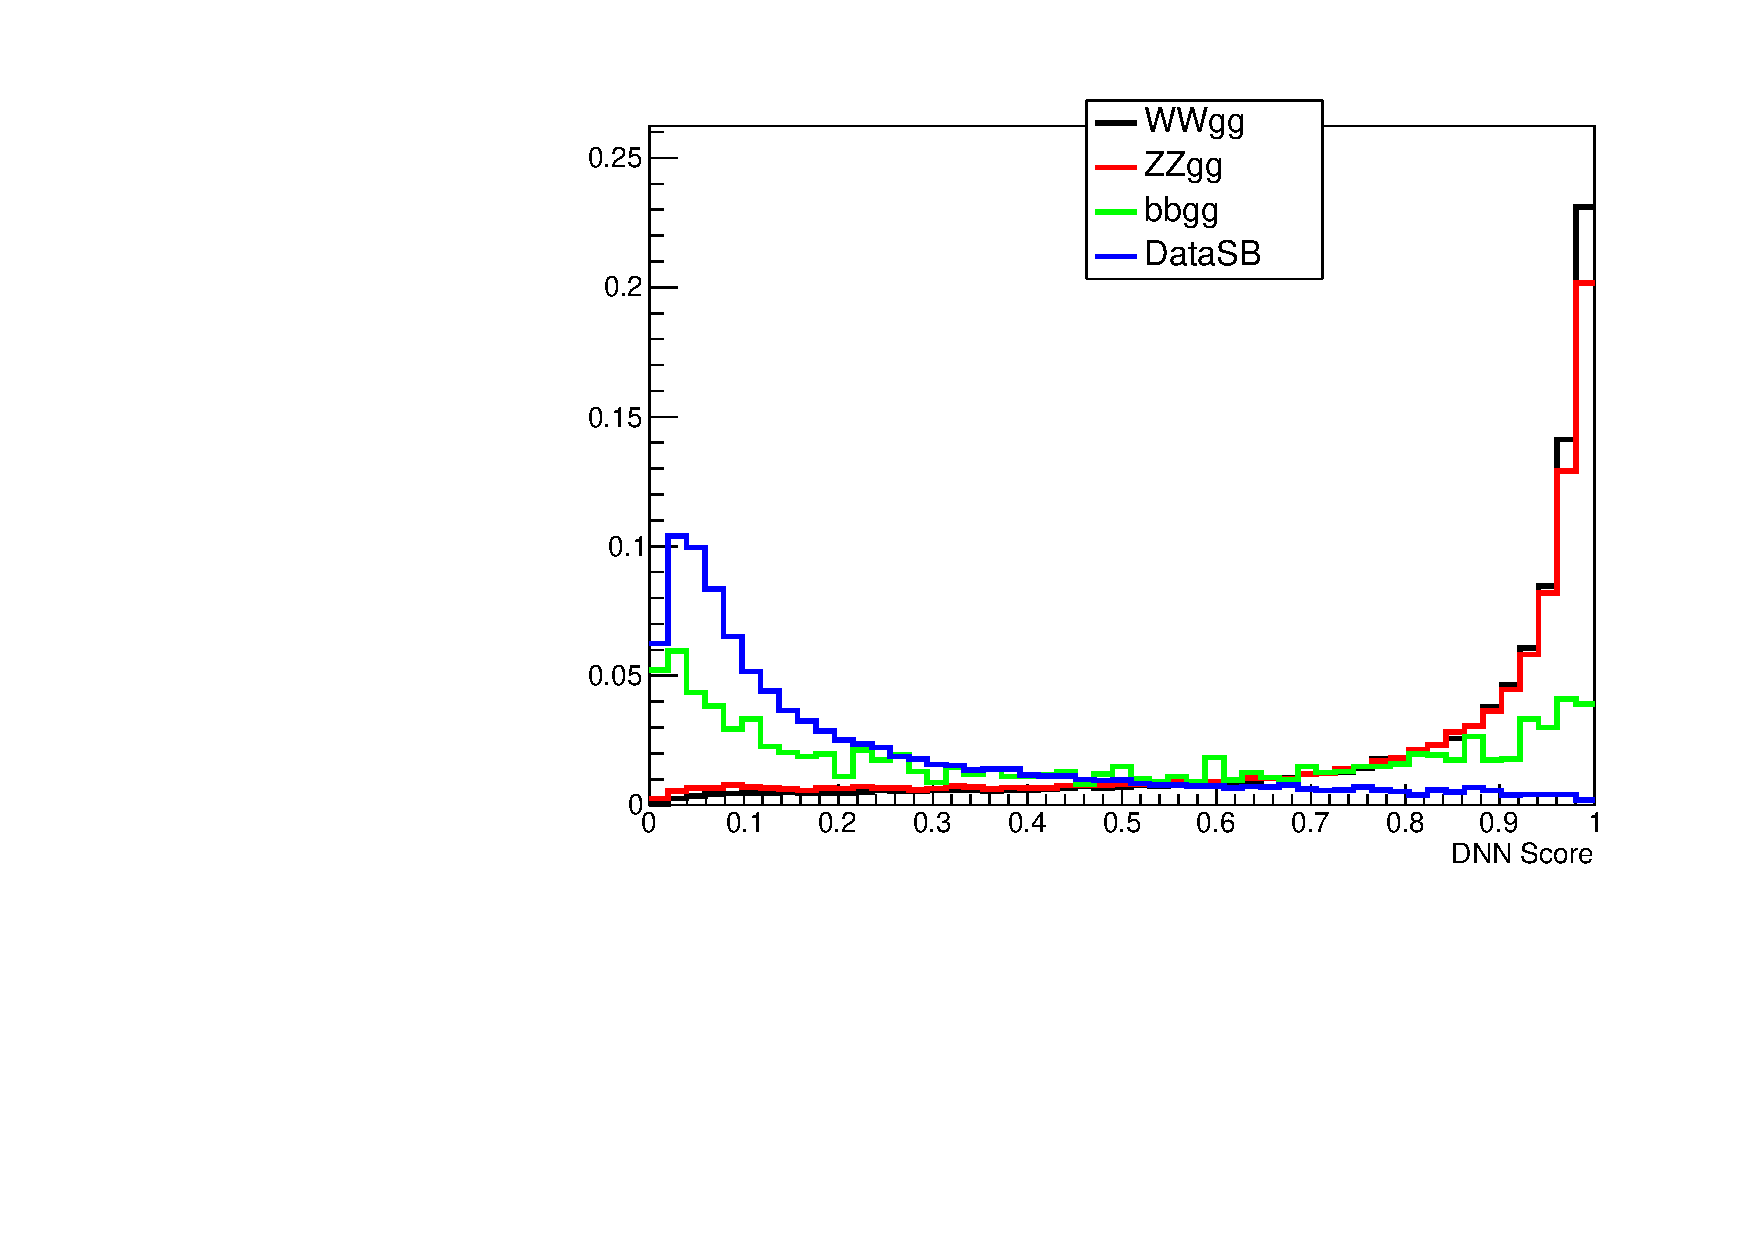
\includegraphics[scale=0.6]{Sections/HHWWgg/images/FH_DNN/WWvsAll_2017_NormUnity_BBggScoreCut0p6.pdf}
  \caption{Fully-Hadronic output score for signal and background. All distributions are normalized to unity.}
  \label{fig:FH_DnnScore}
\end{figure}

These distributions are used for significance computations. 

In performing the categorization, the same method is followed as for the semi-leptonic final state described in Section \ref{subsubsec:SLCategorization}. The result of smoothing of the MC in the signal region is shown in Fig.~\ref{fig:FH_smoothing}.

\begin{figure}[!htbp]
  \centering
  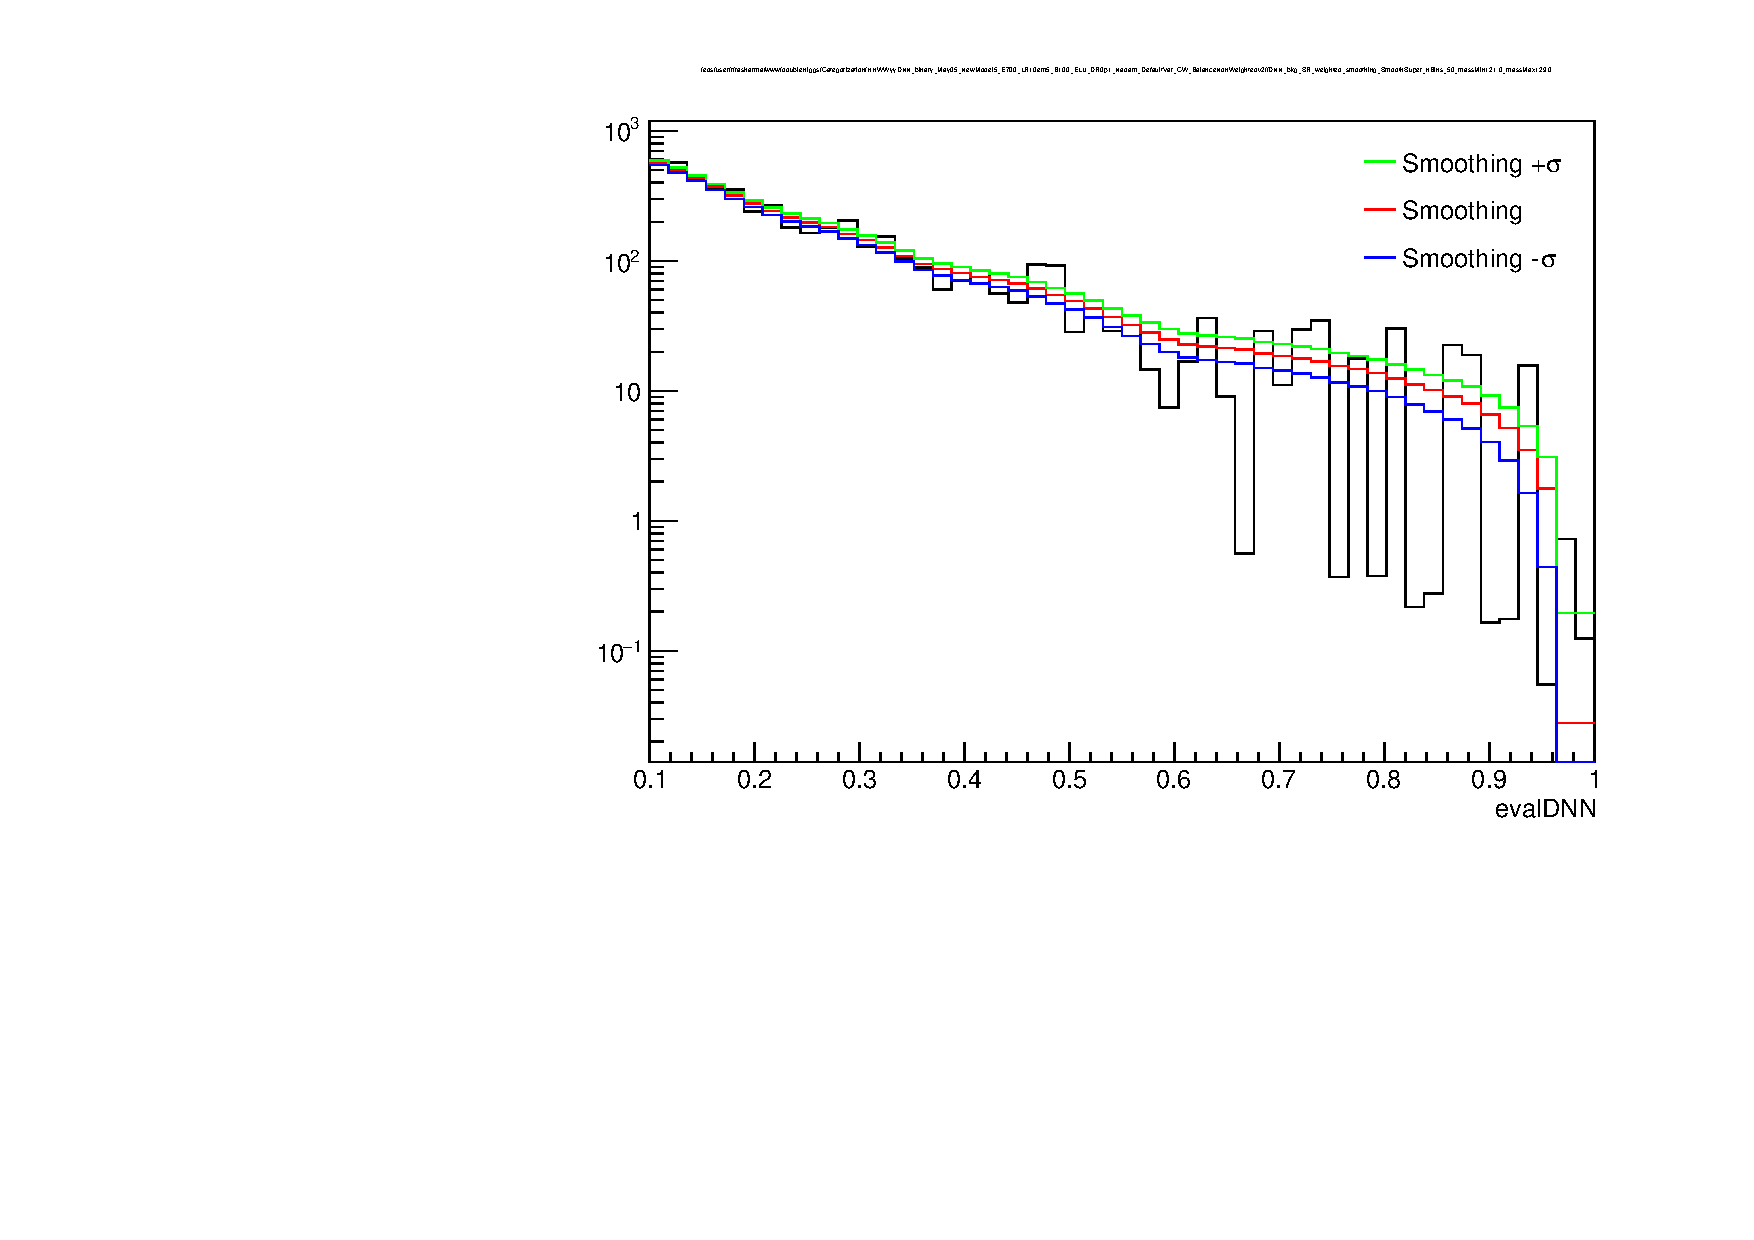
\includegraphics[scale=0.6]{Sections/HHWWgg/images/FH_DNN/h_DNN_bkg_SR_weighted_smoothing_SmoothSuper_nBins_50_massMin121_0_massMax129_0.pdf}
  \caption{Result of background smoothing for Fully-Hadronic channel.}
  \label{fig:FH_smoothing}
\end{figure}

The optimal categorization was chosen based on the 380 bin case, in which category boundaries are simultaneously optimized among 380 equally sized bins of width (1/380) from output WW$\gamma\gamma$ identifier DNN scores of 0.1 to 1.
It was also found that a signal region definition of 120 to 130 GeV in the di-photon mass region returns the greatest significance with number of bins and categories held constant,
a hint that choosing optimal category boundaries based on this definition may return the most sensitive result.
The category boundaries, yields and significance values are summarized in Tab.~\ref{tab:FHcategories_4} for the case of four categories, the final choice on number of categories for optimization.

After categorizing based on the WW$\gamma\gamma$ identifier to maximize signal efficiency, events are required to have a bb$\gamma\gamma$ killer score less than 0.6 in order to remove the majority of bb$\gamma\gamma$ events.

\begin{table}[!htbp]
  \begin{center}
    \begin{tabular}{|c|c|c|c|c|c|c|}
    \hline
    CatN & DNN Min & DNN Max & S        & $B_{SR}$   & $Data_{Sideband}$ & Significance\\ \hline \hline
    0    & 0.983   & 1.0     & 0.03373  & 0.101421   & 24.0              & 0.03373 \\
    1    & 0.969   & 0.983   & 0.04398  & 4.684672   & 55.0              & 0.02029 \\
    2    & 0.893   & 0.969   & 0.13746  & 53.51282   & 384.0             & 0.01878 \\
    3    & 0.1     & 0.893   & 0.30157  & 5979.241   & 27390.0           & 0.00390 \\
    \hline
    \end{tabular}
  \end{center}
\caption{
    Fully-Hadronic DNN Category Boundaries and yields in signal region for 4 Categories
}
\label{tab:FHcategories_4}
\end{table}

